\chapter{Codebase Overview and Responsibility Mapping}

\section{Repository Layout}
The repository root contains two major dimensions: implementation and documentation. Core VPN code resides in \texttt{custom\_vpn/}, while supplementary design notes are in \texttt{docs/}.

\begin{table}[H]
\centering
\caption{Top-Level Structure}
\begin{tabular}{p{0.30\textwidth}p{0.56\textwidth}}
\toprule
\textbf{Path} & \textbf{Purpose} \\
\midrule
\texttt{README.md} & Project overview, quick start, limitations \\
\texttt{custom\_vpn/} & Primary implementation and scripts \\
\texttt{docs/design.md} & Architecture/threat/performance design narrative \\
\bottomrule
\end{tabular}
\end{table}

\begin{figure}[H]
\centering
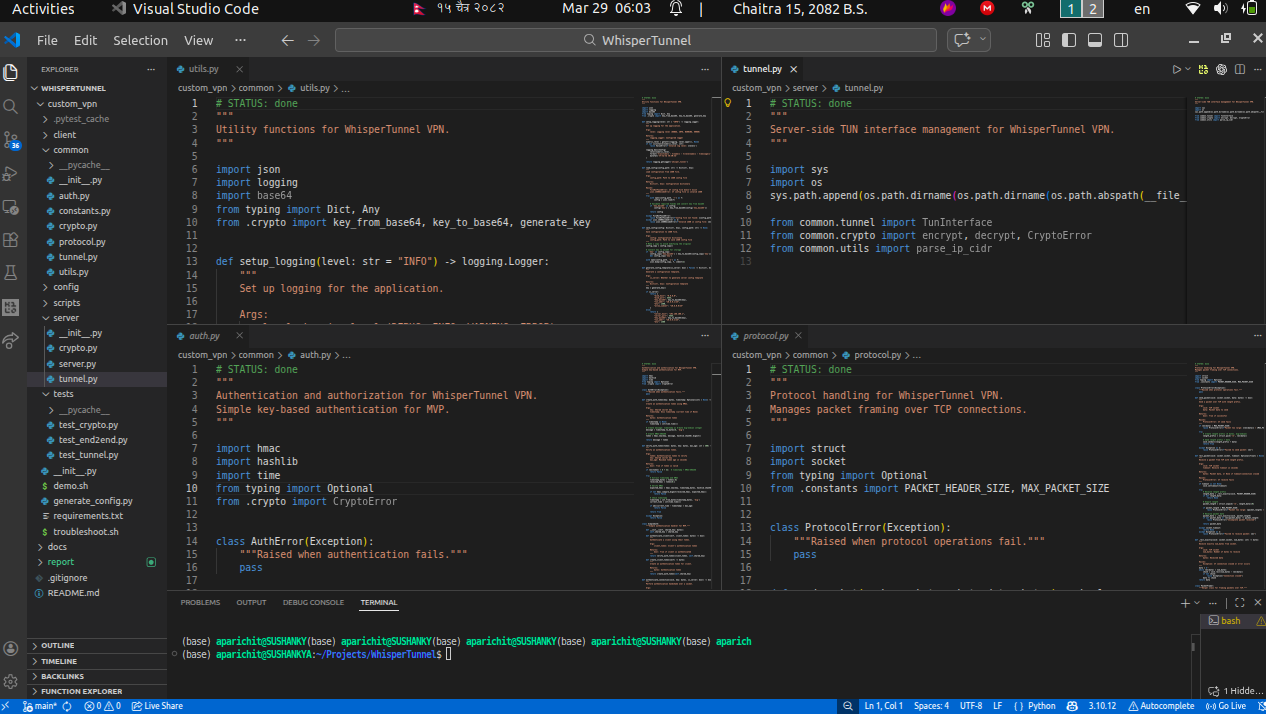
\includegraphics[width=0.95\textwidth]{figures/codebase-shapshot.png}
\caption{Codebase Snapshot}
\label{fig:codebase-snapshot}
\end{figure}

\section{Module Decomposition}
Inside \texttt{custom\_vpn/}, responsibility is layered into shared primitives and endpoint-specific orchestrators.

\subsection{Shared Layer: \texttt{common/}}
\begin{itemize}[leftmargin=2em]
\item \texttt{crypto.py}: AES-GCM encryption/decryption and key conversion.
\item \texttt{protocol.py}: TCP framing and exact-byte receive logic.
\item \texttt{auth.py}: timestamped HMAC token generation and verification.
\item \texttt{tunnel.py}: TUN lifecycle, non-blocking packet I/O, IP configuration.
\item \texttt{utils.py}: config loading/saving, logging, statistics.
\item \texttt{constants.py}: protocol and cryptographic constants.
\end{itemize}

\subsection{Endpoint Layer}
\begin{itemize}[leftmargin=2em]
\item \texttt{client/client.py}: connect/authenticate/setup and bidirectional forwarding.
\item \texttt{server/server.py}: listen/accept/authenticate and forwarding threads.
\end{itemize}

Thin wrappers in \texttt{client/crypto.py}, \texttt{server/crypto.py}, \texttt{client/tunnel.py}, and \texttt{server/tunnel.py} re-export shared functionality and likely exist for organization consistency.

\section{Control Plane and Data Plane Separation}
Code structure naturally separates control actions from packet actions:

\begin{itemize}[leftmargin=2em]
\item \textbf{Control plane}: startup, socket establishment, authentication handshake, thread creation, shutdown handling.
\item \textbf{Data plane}: repeating loops that move packets between TUN and socket with crypto transformations.
\end{itemize}

This split is useful for extension work, because future protocol evolution can be isolated largely to control-plane code while preserving packet loop primitives.

\section{Script Ecosystem}
Operational scripts under \texttt{scripts/} are a major part of usability:

\begin{itemize}[leftmargin=2em]
\item \texttt{netns\_setup.sh}: creates dual namespace topology for local emulation.
\item \texttt{netns\_setup\_internet.sh}: alternative setup with server on host.
\item \texttt{server\_nat.sh}: configures NAT and forwarding rules.
\item \texttt{diagnose.sh}: diagnostics checklist for interfaces/routes/DNS/NAT.
\item \texttt{fix\_internet.sh}: convenience recovery workflow.
\item \texttt{routing.sh}: route rewrite helper.
\end{itemize}

\section{Testing Assets}
The \texttt{tests/} package includes:
\begin{itemize}[leftmargin=2em]
\item Cryptographic behavior tests (round-trip, tamper detection, key validation).
\item TUN interface tests, guarded for root and \texttt{/dev/net/tun} availability.
\item Integration-oriented tests for framing and socket communication.
\end{itemize}

This creates a layered confidence model: pure functions can be validated quickly, while privileged/network tests are opt-in by environment.

\section{Configuration Model}
Configuration is JSON-driven. Client and server files share the same key material using base64 representation:
\begin{itemize}[leftmargin=2em]
\item \texttt{config/client.json}: server endpoint, key, local tunnel address.
\item \texttt{config/server.json}: bind endpoint, key, server tunnel address, allowed subnet hint.
\end{itemize}

The generator script \texttt{generate\_config.py} ensures synchronized key creation for both sides.

\section{Dependency Footprint}
Dependencies are intentionally narrow:
\begin{itemize}[leftmargin=2em]
\item \texttt{cryptography} for AES-GCM operations.
\item \texttt{pyroute2} listed as dependency (not heavily exercised in current code).
\item \texttt{pytest} for test execution.
\end{itemize}

Small dependency surfaces reduce setup complexity for educational use.

\section{Observed Inconsistencies Worth Tracking}
Static inspection reveals a few script-level consistency risks:
\begin{itemize}[leftmargin=2em]
\item Some scripts include Unicode glyphs in output and mixed assumptions about where server runs.
\item \texttt{server\_nat.sh} references \texttt{\$CLIENT\_NS} without local declaration in the visible snippet.
\item Cleanup argument handling in some scripts appears after setup calls, which can cause unintended setup before cleanup.
\end{itemize}

These observations are discussed in risk chapters as operational reliability concerns rather than core protocol flaws.

\section{Summary}
The codebase is compact, understandable, and well suited for educational dissection. Its modular split across \texttt{common/}, endpoint orchestrators, and scripts creates a clear narrative arc for architecture and implementation analysis in the following chapters.
